\chapter{Koordinatensysteme}\label{MULTI-koordinatensysteme}

\begin{table}[H]
  \centering
  \begin{tabularx}{\textwidth}{@{}>{\raggedright\arraybackslash}X r@{}}
    \toprule
    \multicolumn{2}{c}{\textbf{�bersicht �ber Lernziele und Voraussetzungen}}\\
    \midrule
    \textbf{Lernziele} & \\[.5\normalbaselineskip]
    \tabitem geeignete Koordinatensysteme f�r typische Symmetrien ausw�hlen (kartesisch, polar, zylindrisch, kugelf�rmig) & \\
    \tabitem Punkte zwischen kartesischen und Polarkoordinaten umrechnen & \\
    \tabitem Punkte zwischen kartesischen und Zylinderkoordinaten umrechnen & \\
    \tabitem Punkte zwischen kartesischen und Kugelkoordinaten umrechnen & \\
    \tabitem Wertebereiche und Mehrdeutigkeiten der Winkelkoordinaten korrekt ber�cksichtigen & \\[.5\normalbaselineskip]
    \midrule
    \textbf{Voraussetzungen} & \\[.5\normalbaselineskip]
    \tabitem trigonometrische Funktionen &  \\
    \tabitem Polarkoordinaten in $\mathbb R^2$ bzw.\ $\mathbb C$ &  \\
    \bottomrule
  \end{tabularx}
\end{table}

\section*{Leitidee}

Viele Probleme zeigen eine Struktur von Zeilen und Spalten (Kristalle, Solarpanels, Manhattan, \ldots ). F�r diese sind die �blichen kartesischen (\emph{cartesian}) Koordinaten gut geeignet. Viele andere Probleme weisen aber andere Symmetrien auf, insbesondere kreisf�rmige (Rad, Planetenbahn, \ldots ), zylinderf�rmige (Flasche, Tank, \ldots ) oder kugelf�rmige (Erde, Ballon, Tank, \ldots ) und es stellt sich heraus, dass es daf�r geeignete Koordinatensysteme gibt.

\begin{exabox}{Manhatten vs Paris}{ }
	\centering
	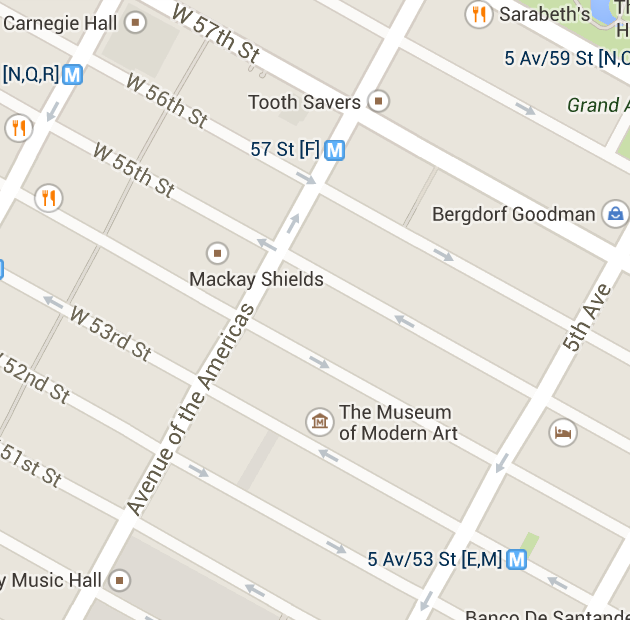
\includegraphics[width=0.3\textwidth]{../Multivariate_Analysis/Bilder/koordinaten_stadtplan_manhattan.png}\hspace{0.5cm}
	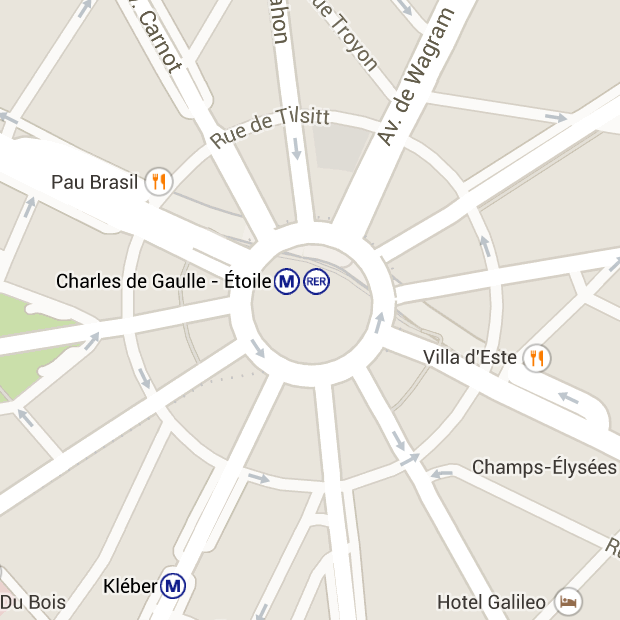
\includegraphics[width=0.3\textwidth]{../Multivariate_Analysis/Bilder/koordinaten_stadtplan_paris.png}
\end{exabox}

W�hlt man Koordinatensysteme, die der Problemstellung angepasst sind, dann k�nnen sich die Problemstellungen enorm vereinfachen! Es gibt drei Koordinatensysteme, die Sie immer wieder brauchen werden. Wir stellen sie jetzt vor.

\section{Polarkoordinaten}

Polarkoordinaten (\emph{polar coordinates}) kennen wir schon von den komplexen Zahlen: Statt einen Punkt im $\mathbb R^2$ als $(x,y)$ zu bestimmen, gibt man seinen Abstand $r$ vom Ursprung und den positiven oder negativen Winkel Azimut (\emph{azimuth}) $\varphi$ zur $x$-Achse an:

\begin{theorembox}{Polarkoordinaten $(r,\varphi)$}{ }
	\begin{minipage}{0.4\textwidth}
		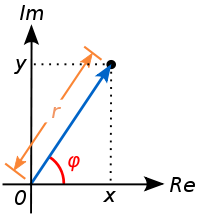
\includegraphics[width=0.7\textwidth]{../Multivariate_Analysis/Bilder/polarkoordinaten_komplexe_ebene.png}
\end{minipage}
\hspace{-2.3cm}\begin{minipage}{0.6\textwidth}
	\begin{itemize}
		\item Der Wertebereich der Koordinaten ist
	\begin{eqnarray*}
		r &\in& [0,\infty)\,,\\
		\varphi &\in& (-\pi,\pi]\,.
	\end{eqnarray*}
\item Umrechnung von Polar- auf kartesische Koordinaten $(r,\varphi) \Rightarrow (x,x)$:
	\begin{eqnarray*}
		x &=& r \cdot \cos(\varphi)\,,\\
		y &=& r \cdot \sin(\varphi)\,.
	\end{eqnarray*}
\item Umrechnung von kartesischen zu Polarkoordinaten $(x,y) \Rightarrow (r,\varphi)$:
	\begin{eqnarray*}
		r &=& \sqrt{x^2 + y^2}\,,\\
		\varphi &=& \mathrm{atan2}(y,x) + n\cdot 2\pi\,.
	\end{eqnarray*}
\end{itemize}
\end{minipage}
\end{theorembox}

\noindent Bemerkungen:\randverweis{MA1-komplexe-zahlen-grundlagen}
\begin{itemize}
	\item der Winkel $\varphi$ ist nur bis auf ein Vielfaches von $2\pi$ bestimmt!
	\item f�r $r=0$ ist der Winkel beliebig!
\end{itemize}

\section{Zylinderkoordinaten}

Man gibt zu den Polarkoordinaten in der $xy$-Ebene die �bliche $z$-Achse dazu und hat damit ein Koordinatensystem f�r den $\mathbb R^3$, die Zylinderkoordinaten (\emph{cylindrical coordinates}):
\begin{theorembox}{Zylinderkoordinaten $(r,\varphi, z)$}{ }
	\begin{minipage}{0.4\textwidth}
		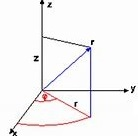
\includegraphics[width=0.7\textwidth]{../Multivariate_Analysis/Bilder/zylinderkoordinaten.png}
\end{minipage}
\hspace{-2.3cm}\begin{minipage}{0.6\textwidth}
	\begin{itemize}
		\item Der Wertebereich der Koordinaten ist
	\begin{eqnarray*}
		r &\in& [0,\infty)\,,\\
		\varphi &\in& (-\pi,\pi]\,,\\
		z &\in& \mathbb R\,.
	\end{eqnarray*}
\item Umrechnung von Zylinder- auf kartesische Koordinaten $(r,\varphi,z) \Rightarrow (x,x,z)$:
	\begin{eqnarray*}
		x &=& r \cdot \cos(\varphi)\,,\\
	y &=& r \cdot \sin(\varphi)\,,\\
	z &=& z\,.
\end{eqnarray*}
\item Umrechnung von kartesischen zu Zylinderkoordinaten $(x,y,z) \Rightarrow (r,\varphi,z)$:
\begin{eqnarray*}
	r &=& \sqrt{x^2 + y^2}\,,\\
	\tan(\varphi) &=& \frac{y}{x}\Rightarrow \varphi = \mathrm{atan2}(y,x) + n\cdot 2\pi\,, \\
		z &=& z\,.
	\end{eqnarray*}
\end{itemize}
\end{minipage}
\end{theorembox}

\section{Kugelkoordinaten}

Die Kugelkoordinaten (sph�rischen Koordinaten) (\emph{spherical coordinates}) sind eine andere Erweiterung der Polarkoordinaten ins Dreidimensionale. Statt der kartesischen $z$-Koordinate wie bei den Zylinderkoordinaten nimmt man hier den Polwinkel (Zenitwinkel) $\theta$ zur positiven $z$-Achse hinzu.
Anders als bei den Zylinderkoordinaten, misst der Radius $r$ den Abstand des betrachteten Punkts vom Ursprung und nicht nur die Projektion in die $xy$-Ebene:

\begin{theorembox}{Kugelkoordinaten $(r,\varphi, \theta)$}{ }
	\begin{minipage}{0.4\textwidth}
		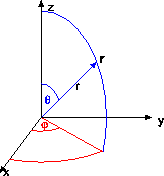
\includegraphics[width=0.7\textwidth]{../Multivariate_Analysis/Bilder/kugelkoordinaten.png}
\end{minipage}
\hspace{-2.3cm}\begin{minipage}{0.6\textwidth}
	\begin{itemize}
		\item Wertebereich f�r Radius, Azimut und Polwinkel
	\begin{eqnarray*}
		r &\in& [0,\infty)\,,\\
		\varphi &\in& (-\pi,\pi]\,,\\
		\theta &\in& [0, \pi]\,.
	\end{eqnarray*}
\item Umrechnung von  $(r,\varphi,\theta)$ auf $(x,x,z)$:
	\begin{eqnarray*}
		x &=& r \cdot \sin(\theta)\cdot \cos(\varphi)\,,\\
		y &=& r \cdot \sin(\theta)\cdot \sin(\varphi)\,,\\
		z &=& r\cdot \cos(\theta)\,.
	\end{eqnarray*}
\item Umrechnung von $(x,y,z)$ auf $(r,\varphi,z)$:
	\begin{eqnarray*}
		r &=& \sqrt{x^2 + y^2 + z^2}\,,\\
		\tan(\varphi) &=& \frac{y}{x} \Rightarrow \varphi = \mathrm{atan2}(y,x) + n\cdot 2\pi\,, \\
		\cos(\theta) &=& \frac{z}{r} \Rightarrow \theta = \arccos\left( \frac{z}{r}\right) \,,
	\end{eqnarray*}
\end{itemize}
\end{minipage}
\end{theorembox}

